\chapter{Einleitung}

In einer vernetzten Welt senden Geräte Daten über ihren Zustand oder der, ihrer Umgebung. Diese Technologie wird für ein Fahrradfahrer nutzbar gemacht. Das Handy soll die aktuelle Geschwindigkeit, die Höhe über dem Meer, die Temperatur und die Luftfeuchtigkeit während der Fahrt empfangen.

Diese Idee ist nicht neu. Erhältlich sind batteriebetriebene Modelle, die Daten auf einem Display anzeigen. Das Neue an dieser Arbeit ist, dass die Energie aus der Fahrradumdrehung geerntet wird und dass der User sein eigenes Handy für das Anzeigen der Daten nutzen kann.


\section{Ausgangslage}

Als Inspiration dienten zwei batteriebetriebene Modelle der Hersteller Sigma Sport und Polar. Sigma Sport bietet Geräte mit eigenem Display und  Sensoren an. Auf dem Display erscheint neben der Geschwindigkeit, die Daten der Sensoren, die GPS-Ortung und den aktuellen Ladestand der Batterie. Der Hersteller Polar stellt ein Gerät her, welches die Fahrt über GPS aufzeichnet und wichtige Informationen zur Trainingsverbesserung liefert. Als Nachteil bewerteten wir, dass ein (verdrahtetes) Display gebraucht wird.

Während der Arbeit wurden wir auf den Hersteller Reelight aufmerksam. Reelight gewinnt über Wirbelströme Energie und schafft es bei seinem Produkt City Supreme genügend Energie für eine LED-Lampe zu erzeugen. Da auf der Webseite keine Dokumentation des Funktionsprinzips erhältlich ist, ergaben eigene Untersuchungen, dass sich im Innern der Lampe \glqq etwas\grqq bewegt. Unserer Meinung nach ist dies ein Magnet, der so gelagert ist, dass er sich drehen kann. Der an der Felge vorbeiziehende Magnet erzeugt ein Wirbelstrom auf der Felge. Dieser wirkt auf den Magneten im Licht und der Magnet im Licht beginnt sich zu drehen. Befindet sich neben dem sich drehenden Magneten eine Spule, so wird genügend Spannung für das Betreiben einer LED induziert. Diese Harvesting-Methode beurteilen wir als interessant für eine zukünftige Arbeit. Der Nachteil dieser Methode ist, dass das Erzeugen eines Wirbelstroms auf den Felgen bremsend wirkt.  Bei dieser Bachelorarbeit war die Harvesting-Methode bereits vorgegeben, da sie auf einer vorangehenden Projektarbeit basiert.

Als Grundlage dient der Aufbau aus der Machbarkeitsstudie\glqq  Bicycle computer and sensoric powered with harvested energy\grqq (\cite{PA_bicycle}). In dieser Projektarbeit wurde der Beweis erbracht, dass durch Bewegungsinduktion genug Energie erzeugt werden kann, um die Geschwindigkeit des Fahrrads per Bluetooth Low Energy zu übermitteln. Der Aufbau funktioniert nach vorangehendem Laden der Kondensatoren zuverlässig bei 20 km/h. Das Ziel dieser Arbeit besteht aus einer verbesserten Energiegewinnung, einem besserem Verbrauchsmanagement und einer ansprechenden Applikation. Konkret soll ein attraktives Produkt ohne Aufladen der Kondensatoren für eine Geschwindigkeit bei 10 km/h entstehen. Diesen Prototypen wird in dieser Arbeit kurz Bicycle Computer genannt.



\section{Definition der Aufgabenstellung}\label{Aufgabenstellung} 

Durch die offiziellen Ausschreibung der Bachelorarbeit an der ZHAW ist der Inhalt der Bachelorarbeit vorgegeben (siehe Anhang \ref{Ausschreibung}). Das Ziel der Arbeit ist, aus dem Aufbau einer Machbarkeitsstudie einem Prototypen eines batterielosen Fahrradcomputers zu entwickeln. In den ersten Sitzungen zusammen mit Prof. Dr. Marcel Meli und Herr Dario Dündar wurde die Aufgabenstellung auf folgende Punkte konkretisiert:

\begin{enumerate} 

\item Inbetriebnahme des Prototypen, Einlesen in die vorangegangene Projektarbeit und Beschäftigung mit der Materie, sind die Hauptpunkte des ersten Schrittes.
\item Die bestehende Hardware muss verkleinert und überarbeitet werden. Dafür wird ein neues PCB entworfen, welches verschiedene vorhandene Platinen vereint.
\item Initialisierung der Bluetooth-Schnittstelle muss auf dem Android-Endgerät und der Hardware vorgenommen werden. Eine erste Bluetooth-Kommunikation zwischen der Hardware und der Applikationen ist implementiert.
\item Das bestehende Energiemanagement soll auf die Anwendung eines Fahrradcomputers optimiert werden.
\item Die Benutzeroberfläche der Android-Applikation soll benutzerfreundlich und optisch ansprechend gestaltet werden.
\item Die erfassten Messwerte der Geschwindigkeit und der aktuellen Höhe sollen über Bluetooth übermittelt werden.
\item	Die erfassten Daten sollen gespeichert und nur dann übertragen werden, wenn die nötige Energie vorhanden ist.
\item	Per GPS soll die aktuelle Position ermittelt, sowie die bereits abgefahrene Route erfasst werden. Alles soll auf einer Karte veranschaulicht werden.
\item	Die Beschleunigung, Luftfeuchtigkeit und Temperatur sollen ebenfalls erfasst und über Bluetooth übermittelt werden.
\item	Das Energiemanagement soll für verschiedene Geschwindigkeiten optimiert werden.
\end{enumerate}

Bei der Festlegung der Arbeitsschritte half die Vision eines innovativen Fahrradcomputers. Die Miniaturisierung (Punkt 2) ist für die Attraktivität des Produkts entscheidend. Ebenso beurteilen wir es als Vorteil, das eigene Handy als Display für die Daten zu verwenden. Aus diesem Grund wurde Punkt 5. zu den wesentlichen Aufgaben genommen. Die App soll ansprechend und einfach für die Benutzerin oder den Benutzer sein. Das verbesserte Energy Management (Punkt 4) hat mit dem Ziel zu tun, dass der Fahrradcomputer bereits bei 10 km/h die Geschwindigkeit ausgeben soll. So gelten für die Bachelorarbeit die Punkte 1.) bis 6.) als Minimalanforderungen, während die Punkte 6) bis 10) dynamisch und in Abhängigkeit des Projektfortschritts einbauen lassen. Aus den definierten Anforderungen entstand der auf der CD abgelegte Projektplan.

\section{Übersicht der Aufgabenblöcke}

Um den Überblick der zu erledigenden Punkte zu behalten, werden die Aufgaben in Arbeitsblöcke (siehe Abbildung \ref{arbeitsbloecke} ) geteilt. Die gepunkteten Blöcke sind optional, die voll umrandeten entsprechen dem Minimum.Die Projektplanung wurde so aufgebaut, dass bei Meilenstein 1, das Layout gezeichnet ist, bei Meilenstein 2 die Kommunikation zur App besteht, bei Meilenstein 3 die überarbeitete Version des Prototyps gezeigt wird und bis dahin das Minimum erreicht ist. Welche optionalen Ziele realisiert werden, wird im Meilenstein 3 definiert.

\begin{figure}[ht]
    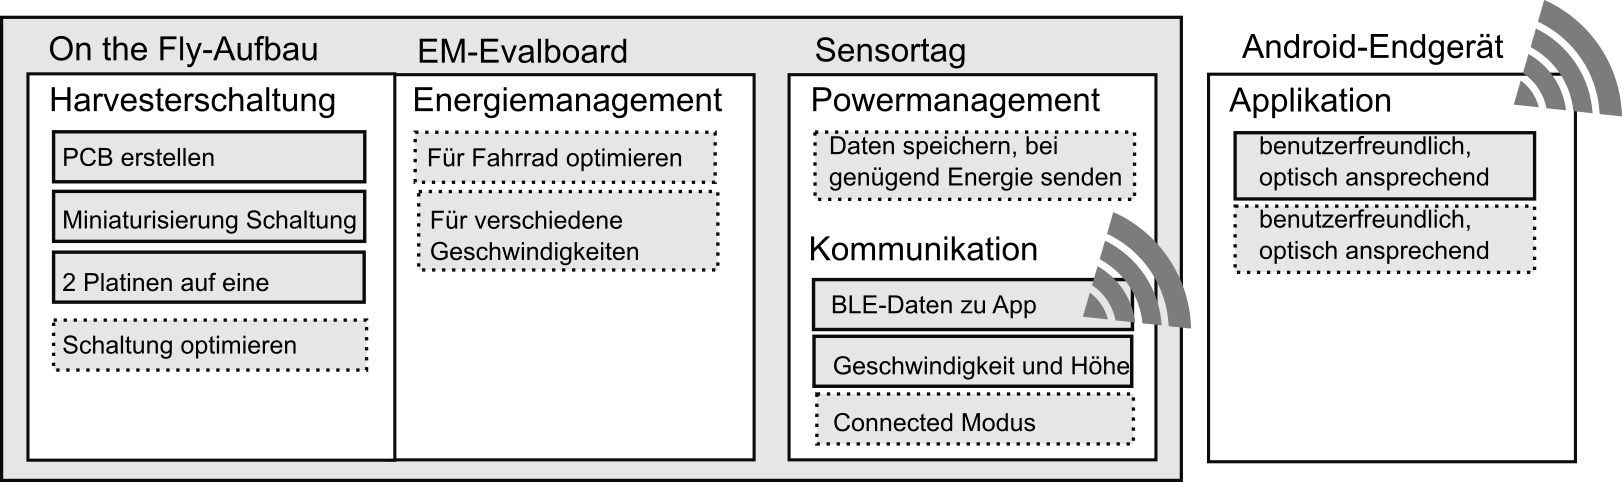
\includegraphics[width=1.0\textwidth]{../ressources/Projektorganisation/Arbeitsbloecke.png} 
    \caption{Arbeitsblöcke}
\end{figure}\label{arbeitsbloecke} 

